\section{Zweite Evaluation}
In der zweiten Evaluation werden drei Lösungsvarianten in einem morphologischen Kasten dargestellt. Anschliessend werden diese Lösungsvarianten in einer Nutzwertanalyse bewertet.
\subsection{Morphologischer Kasten}
In der ersten Phase der zweiten Evaluation werden die Ergebnisse der ersten Evaluation in einem morphologischen Kasten zusammengefasst. Mithilfe dieses morphologischen Kastens werden drei mögliche Lösungskonzepte zusammengestellt. Hierbei wird sich an der Teilfunktion ``Treppensteigen'' orientiert. Nach dem ersten Schritt, werden die restlichen Komponenten hinzugefügt. Die Hauptunterschiede dieser drei möglichen Lösungskonzepte (Frosch, 3-teiliger Hebemechanismus, Beine) liegen bei den Teilfunktionen: Treppensteigen, Lenkung und Fortbewegung.

Frosch: Ziel der ersten Variante ist es, einen möglichst einfachen Roboter zusammenzustellen, welcher speziell bei den kritischen Teilfunktionen simpel und zuverlässig funktioniert. So wird hier das Roomba-Lenkungsprinzip mit zwei angetriebenen Rädern verwendet. Das bedeutet weniger Komponente, Gewicht und Entwicklungsaufwand. Da die Funktionen mehrheitlich vom Treppensteigen-Mechanismus abhängig sind, ergeben sich das Zugmittelgetriebe, Akku und Elektromotoren selbsterklärend.

Hebemaschine: Bei der Variante 2, geht es um eine 3-Teilige Hebemaschine, welche sich sektionsweise hebt, um auf die nächste Stufe zu gelangen. Aufgrund der zu erwartenden Grösse, wird ein Omnidrive-Fahrmodul eingeplant. Somit kann sich der Roboter um die Hindernisse herum verschieben, ohne sich um seine eigene Achse drehen zu müssen. Um die Treppenstufen zu erklimmen wird ein Hebemechanismus verwendet, welche zwingend Getriebe und Elektromotoren voraussetzt.

Beine: Bei der dritten Variante wird ein Roboter zusammengestellt, welcher auf Beinen läuft. Dabei muss keine Lenkung verbaut werden. Auch eine Treppensteigfunktion wird nicht verwendet, da dieser Roboter mit den Beinen alleine in der Lage ist, die Treppen zu erklimmen. Für die Fortbewegung werden einzig Elektromotoren und Akkus verwendet.

Unabhängig vom Treppensteig-Mechanismus und vom Robotertyp selbst sind neben den Steuerungseinheiten auch die Kommunikation und die Umgebungserkennung. Das hauptsächlich, da es bei allen Robotern gleichermassen vorhanden sein muss. Bei der Steuerungseinheiten wird Raspberry und Arduino im Vordergrund stehen. Dies aufgrund der bewährten Zuverlässigkeit und Einfachheit. Ebenfalls aufgrund der bereits vorhandenen Erfahrung mit diesen Entwicklerboards. Die Kommunikation wird über Buzzer oder 5V-Lautsprecher in Verbindung mit LEDs getätigt. Mit einziger Ausnahme von Variante 3, sie verzichtet auf die LED und verwendet dafür ein LCD Display.

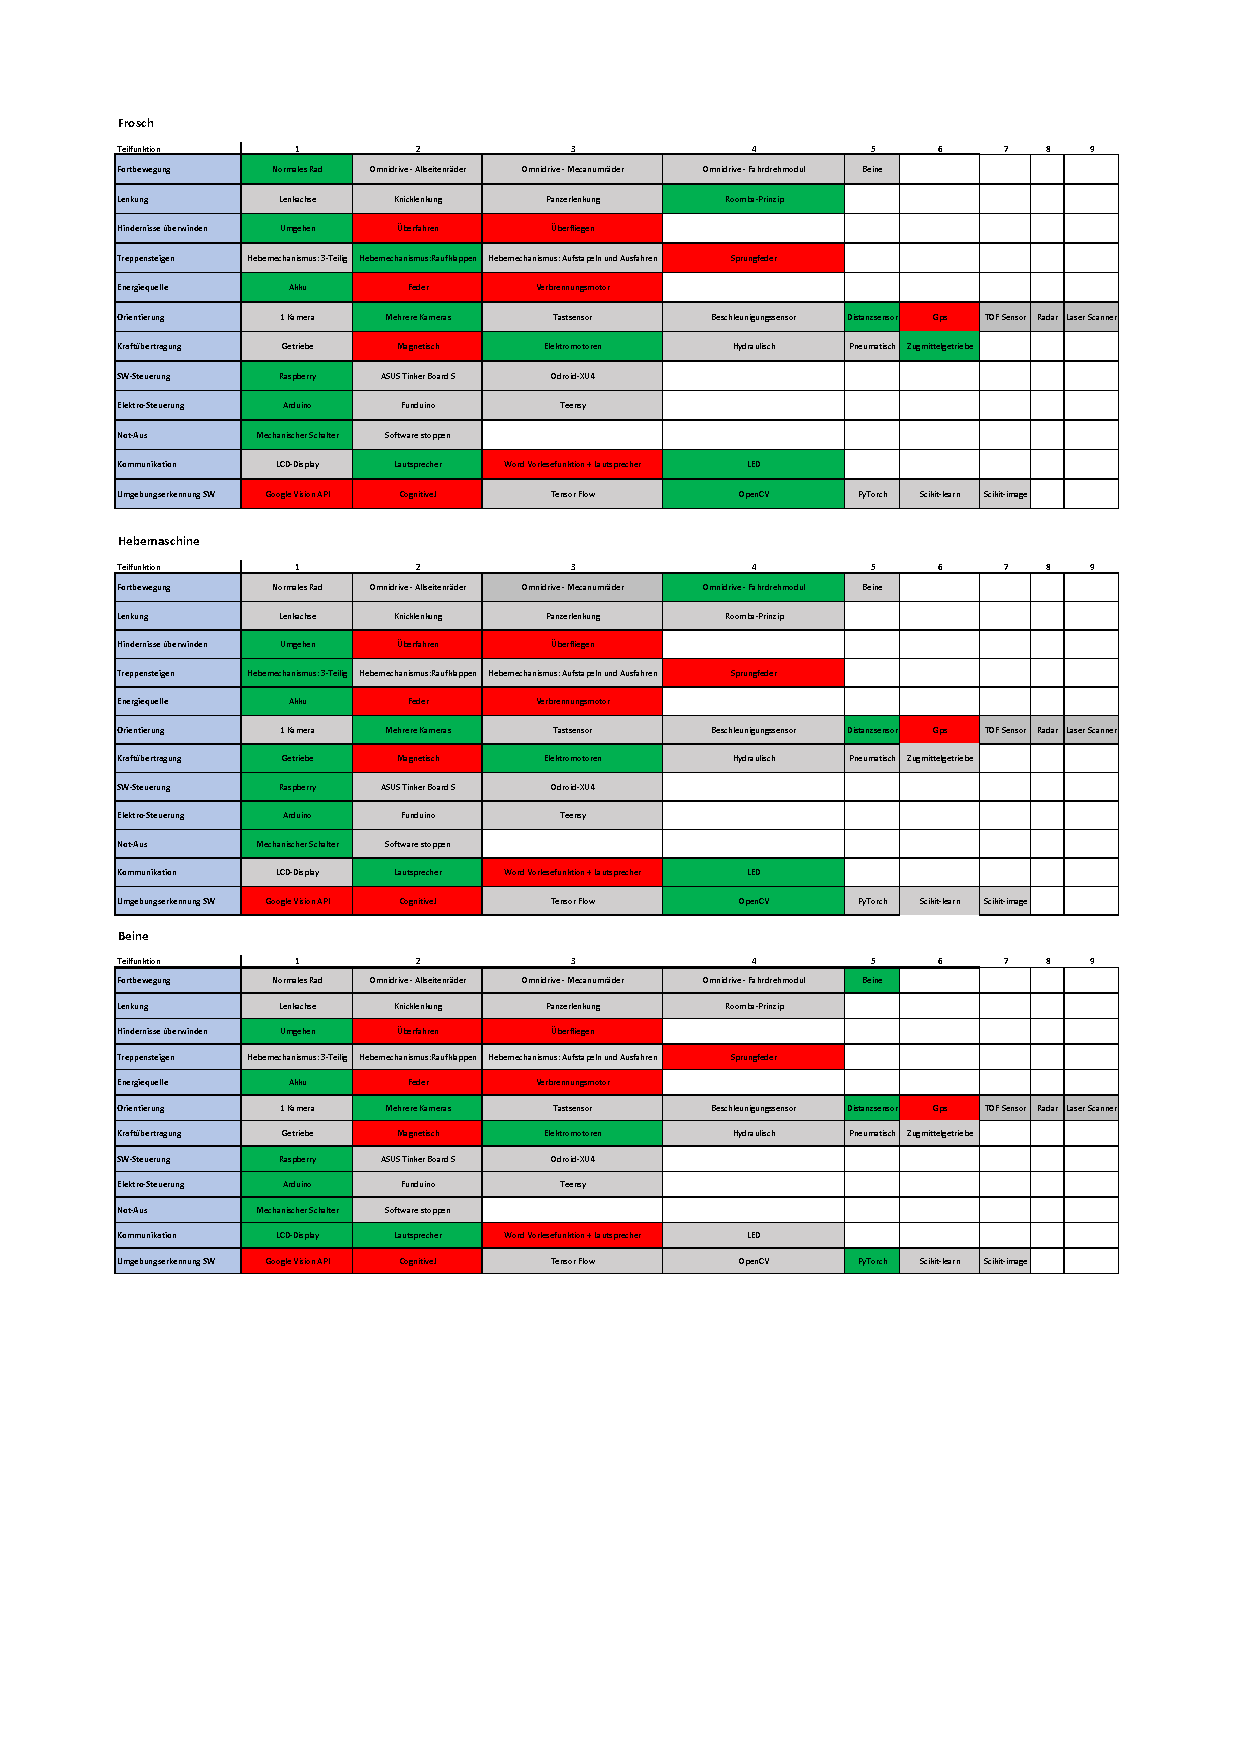
\includepdf[
  pages={1-},
  scale=1,
  pagecommand={\pagestyle{fancy}}
]{assets/MorphologischerKasten.pdf}


\subsection{Nutzwertanalyse}
In der zweiten Phase werden drei möglichen Lösungskonzepte anhand einer Nutzwertanalyse miteinander verglichen. Wichtige Kriterien sind hierbei unter anderem der Entwicklungsaufand, die Zuverlässigkeit, die Geschwindigkeit aber auch die Kosten. 

Aufgrund der Auswertung der nachfolgenden Nutzwertanalyse wird die Variante 1, ``Frosch'', als die geeignetste Variante hervorgehoben. Der Frosch überragt die anderen Varianten in nahezu allen Systemkritischen Kategorien. Eine Ausnahmen ist der Not-Aus, welcher bei allen Varianten identisch ist und dementsprechend auch bei der Nutzwertanalyse bei allen gleich ausfällt. Die andere Kategorie ist die der Umgebungserkennung, bei welcher die Variante 3 knapp besser abschneidet. Die Zusammenstellung der Umgebungserkennung ist jedoch noch nicht definitiv, da erst einige Test mit Machine-learning durchgeführt wurden. Eine Definitive Aussage, welches Verfahren in diesem Bereich zuverlässiger und geeigneter ist für dieses Projekt kann erst nach weiteren Test zuverlässig gemacht werden.

Aufgrund der Bewertungen dieser Nutzwertanalyse, wird die Variante 2, ``3-Teiler'', als Notfallplan definiert. Falls es im weiteren Verlauf grundlegende Probleme mit der ersten Wahl geben sollte, welche nicht behoben werden können, wird auf diese Variante ausgewichen.

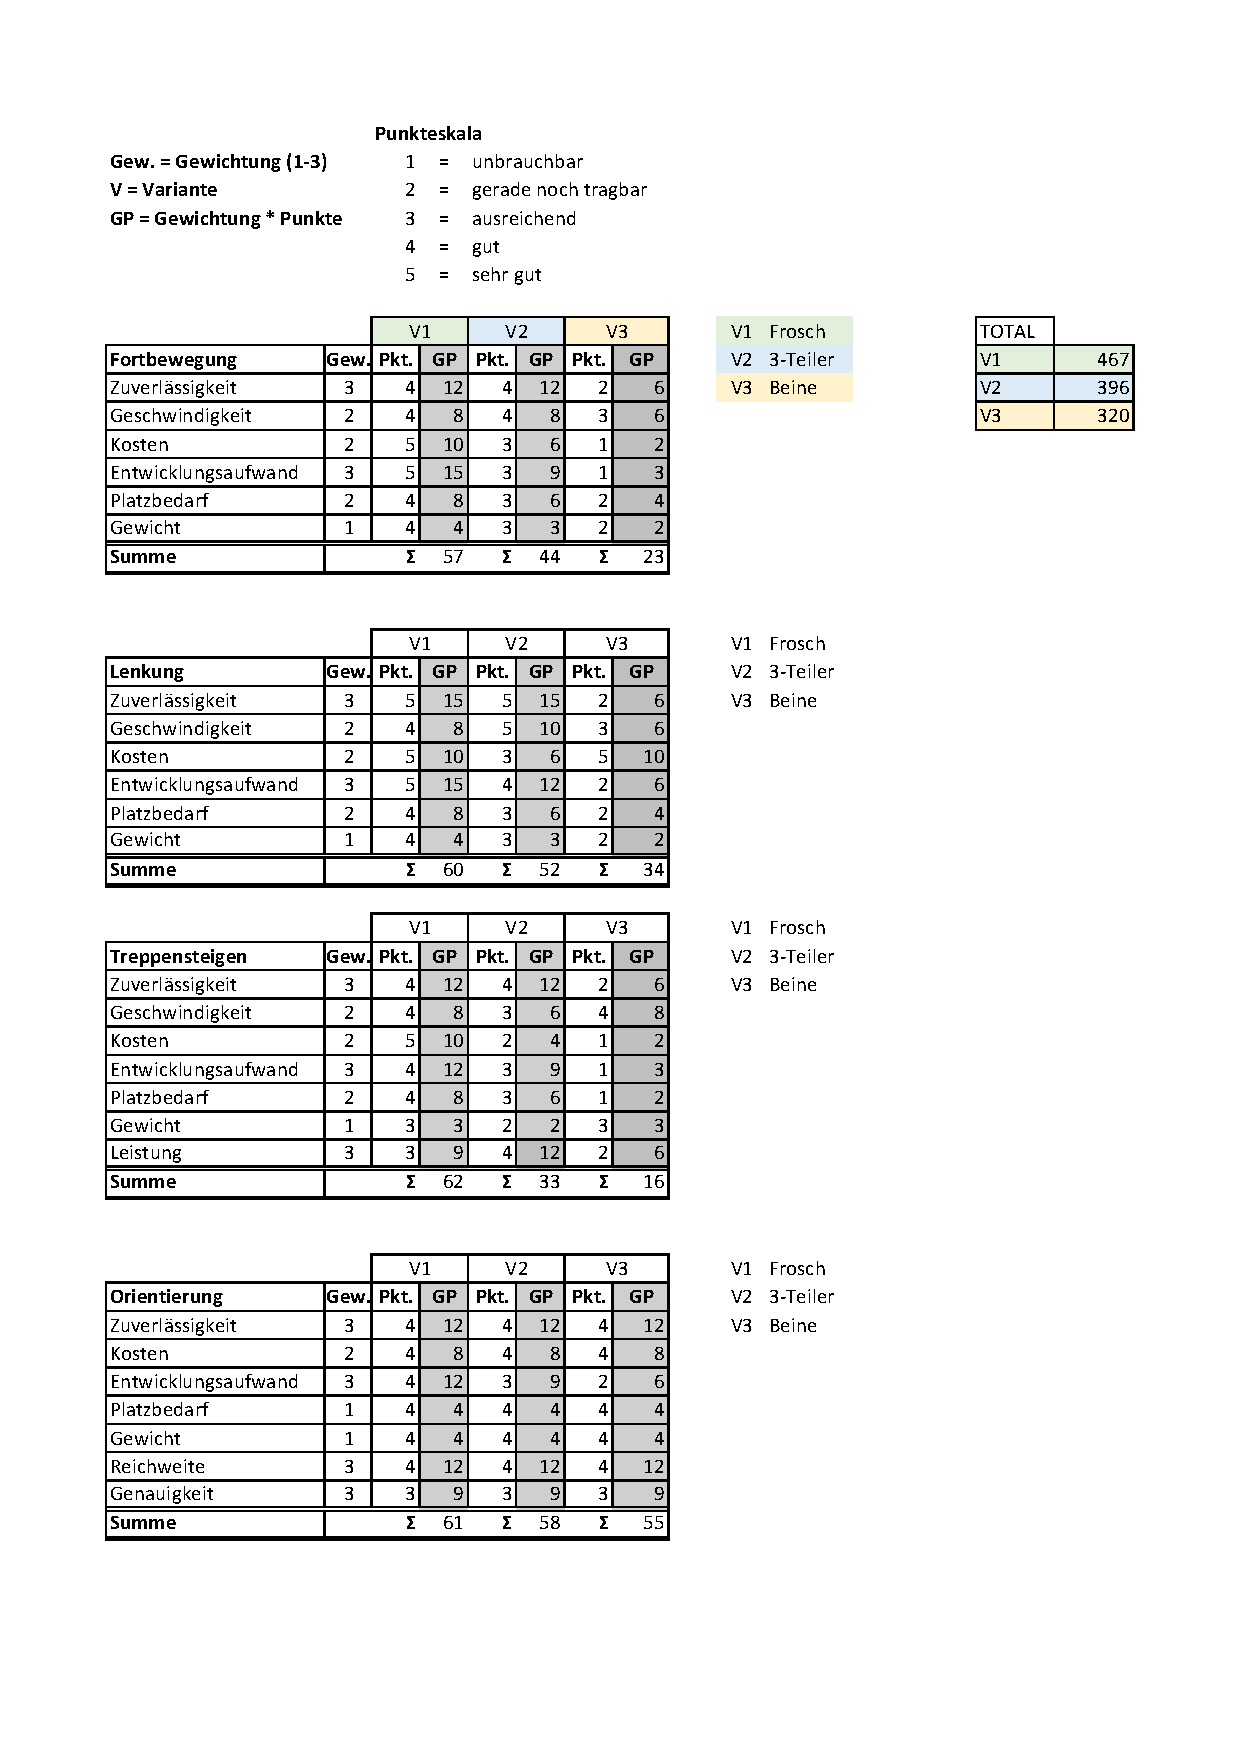
\includepdf[
  pages={1-},
  scale=1,
  pagecommand={\pagestyle{fancy}}
]{assets/Nutzwertanalyse.pdf}

\captionlistentry[table]{Nutzwertanalyse}

\subsection{Komponenten Übersicht der gewählten Lösungskombinationen}
Nachfolgend ist eine Übersicht der Komponenten des erst- und zweit-platzierten Lösungskonzept zu sehen. Für das erstplazierte Lösungskonzept wurde eine Skizze zu den Teilfunktionen Treppensteigen und Fortbewegung erstellt.


\vspace{3cm}

\image
   {img/Skizze Frosch.png}
   {Skizze Treppensteigfunktion und Fortbewegung des Frosches}

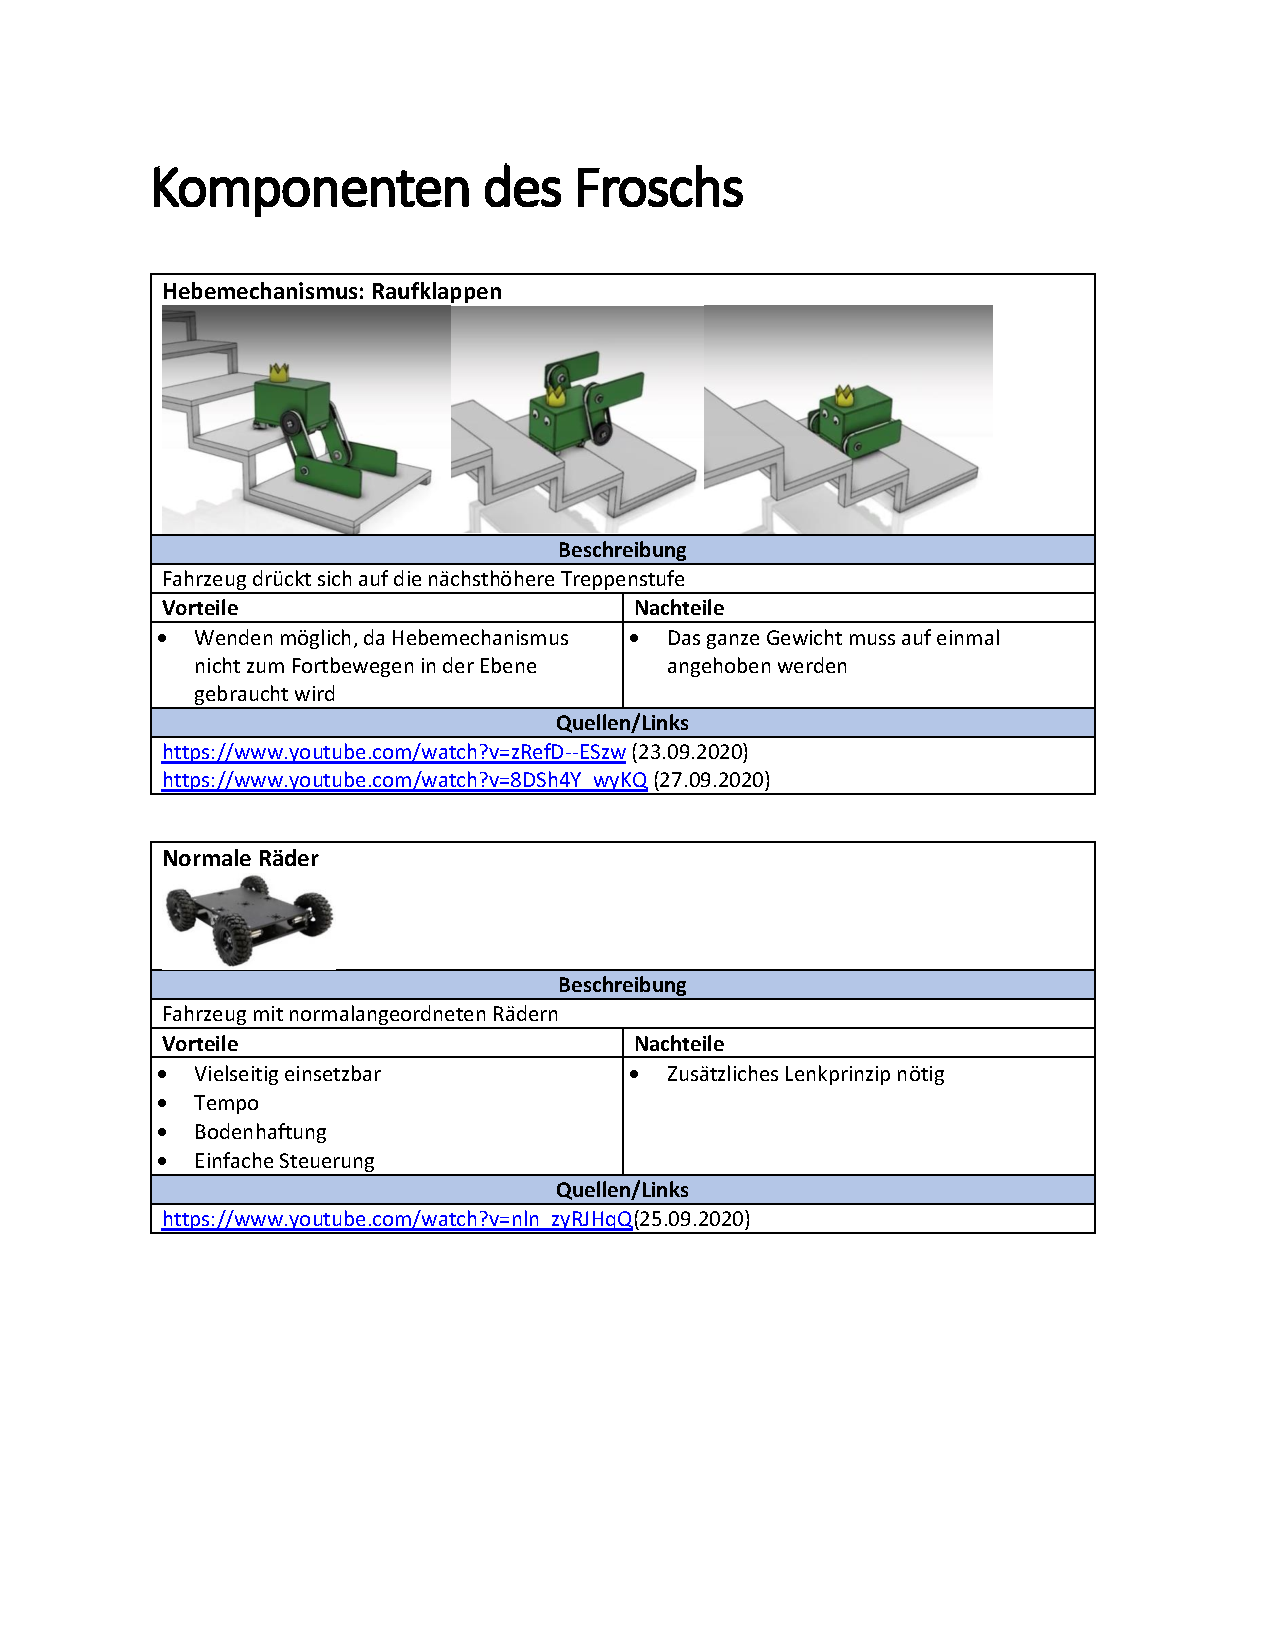
\includepdf[
  pages={1-},
  scale=1,
  pagecommand={\pagestyle{fancy}}
]{assets/Komponenten Frosch.pdf}

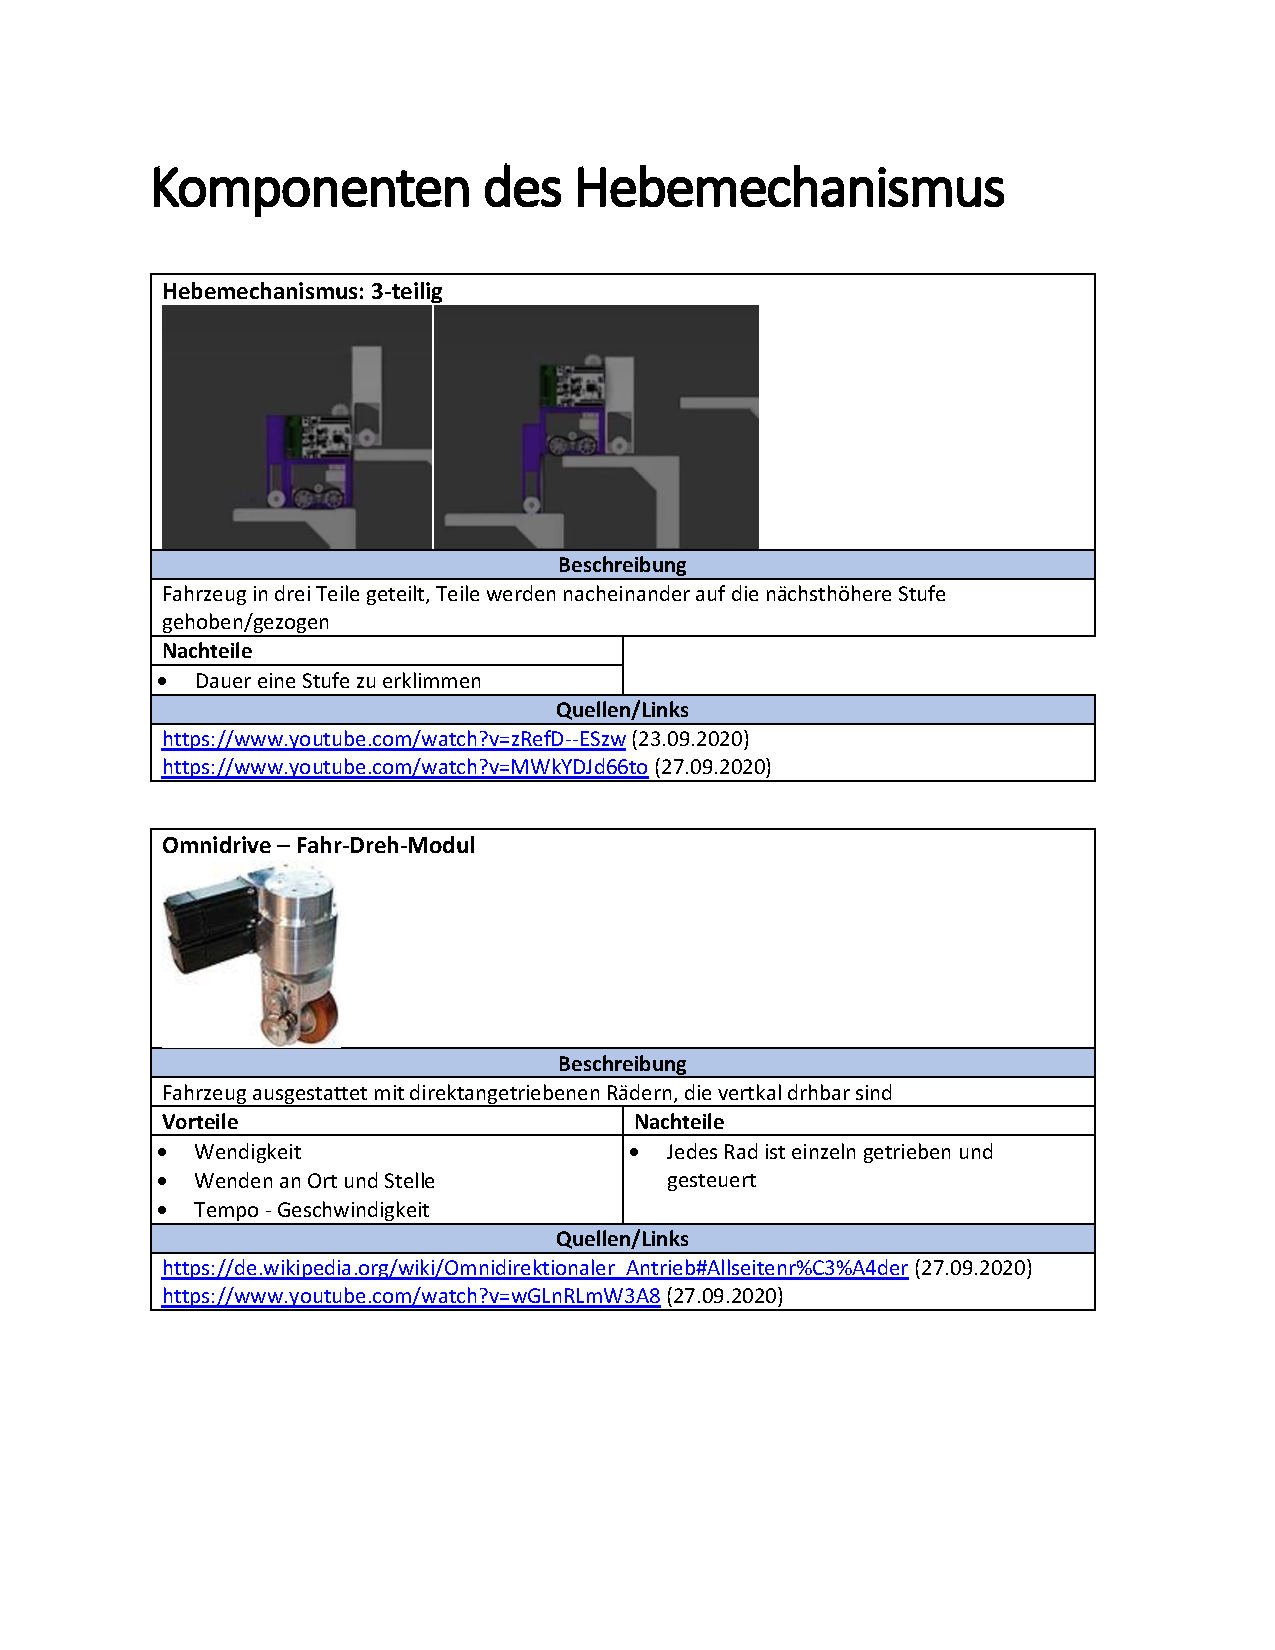
\includepdf[
  pages={1-},
  scale=1,
  pagecommand={\pagestyle{fancy}}
]{assets/Komponenten Hebemechanismus.pdf}

\subsection{Mock-Up}
 
 Es wurde ein Mock-Up mit den ersten Massabschätzungen 1:1 erstellt. Das Mock-Up wurde aus Lego und Karton aufgebaut. Die ersten Massabschätzungen wurden anhand des Datenblatts der Treppe getroffen. Mit diesem Mock-Up wollte getestet werden, ob die Treppensteigfunktion funktioiniert, mit dem Treppensteigprinzip, das anhand der Nutzwertanalyse das Beste ist. Auf einer aus Holz selber gebauten Treppe wurde die Hubbewegung von Hand getestet.
 Ziel ist es dieses Mock-Up als Grundlage für einen Prototypen zu verwenden, der die Hubbewegung automatisch ausführt.
 
 \imagewidth
   {img/modell_treppe_1.png}
   {Eigenes Treppenmodell}
   {0.5\textwidth}

 \image
   {img/stufenerklimmung.png}
   {Mockup für die Stufenerklimmung}